% !TeX spellcheck = en_US
\documentclass[aspectratio=1610]{beamer}
\mode<presentation>
{
  \usetheme{Boadilla}
  \setbeamercovered{transparent}
  
  \definecolor{cobalt}{rgb}{0.0, 0.02 0.50}
  
  \usecolortheme[named=cobalt]{structure}
  %\usecolortheme{lily}
  %\setbeamercolor{headline}{fg=cyan!80!black}
  % \setbeamercolor{frametitle}{bg=white}.
}

\makeatletter
\define@key{beamerframe}{wide}[10pt]{%
	\def\beamer@cramped{\itemsep #1\topsep0.5pt\relax}}
\makeatother
	

\usepackage[english]{babel}
\usepackage[utf8]{inputenc}
\usepackage{times}
\usepackage[T1]{fontenc}
\usepackage{array}
\usepackage{xcolor}
\usepackage{colortbl}
\usepackage{booktabs}

\title[Fall - Lecture 3] % (optional, use only with long paper titles)
{Macroeconomic Theory and Policy: Lecture  3 (Ch.3)}

\author[University of Toronto] % (optional, use only with lots of authors)
{}
\date[] % (optional, should be abbreviation of conference name)

\begin{document}

\begin{frame}
  \titlepage
\end{frame}

\begin{frame}[wide]{What are You Going to Learn (ch. 3)}
	\begin{itemize}
		\item Some facts related to economic growth that later chapters will seek to explain
		\item The substantial improvement of global welfare brought about by economic growth
		\item How this growth is a relatively recent phenomenon
		\item Tools employed to examine economic growth, e.g., growth rate computation
		\item The rationale behind utilizing a "ratio scale" to facilitate the comprehension of per capita GDP plots
	\end{itemize}
\end{frame}

\begin{frame}[wide]{Motivation: Why Is Economic Growth Important?}
	\begin{itemize}
		\item A 1 percent change in annual growth appears small, but it may lead to large differences in the levels of output over time
		\item Consider a 100-year period:
		\begin{itemize}
			\item Country A and B begin at the same level of GDP (\$100 billion)
			\item Country A grows at 1 percent each year
			\item Country B grows at 0.25 percent each year
		\end{itemize}
		\begin{figure}
			\centering
			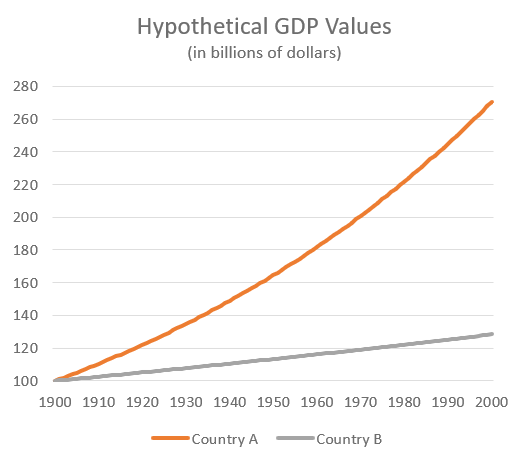
\includegraphics[width=0.4\linewidth]{Figures/growth_100_vs_025}
		\end{figure}
	\end{itemize}
\end{frame}

\begin{frame}[wide]{Motivation: Why Is Economic Growth Important?}
	\begin{itemize}
		\item Many developed countries of a century ago could be mistaken for a emerging country today
		\begin{itemize}
			\item Most of human history has been characterized by little to no economic growth
			\item The last two to three centuries are different than other periods in history in that people lived beyond subsistence levels
		\end{itemize}
		\item 	The study of economic growth explains differences between countries and differences over time
		\begin{itemize}
			\item For example, why is GDP in the United States higher than in Bangladesh?
			\item Or, why have standards of living increased in the United States over time, despite the severity of the many recessions?
		\end{itemize}
	
	\end{itemize}
\end{frame}

\begin{frame}[wide]{Motivation: Why Is Economic Growth Important?}
	\begin{itemize}
		\item 	Even if a country is experiencing a recession, countries with higher levels of GDP still have higher standards of living
		\vspace{3mm}
		\item Economic growth and standards of living are not a short-term result (even though business-cycle fluctuations can affect welfare)
		
	\end{itemize}
\end{frame}

\begin{frame}[wide]{Growth Over the Very Long Run}
	\begin{itemize}
		\item Sustained increases in standards of living are a recent phenomenon:
		\begin{itemize}
			\item The first agricultural revolution was about 10,000 years ago -- humans were hunters and gatherers
			\begin{itemize}
				\item Wages in ancient Greece and Rome were approximately equal to wages in Britain in the fifteenth century or France in the seventeenth century (prior to modern economic growth)
			\end{itemize}
			\item Yet, only in the last 200–300 years has modern economic growth appeared -- urbanization and mechanized
			\begin{itemize}
				\item 200-300 years is long, but relatively short for human history
			\end{itemize}
		\end{itemize}
		\item Economic growth emerges in different places at different times for many reasons.  Some results of this are:
		\begin{itemize}
			\item Standards of living have diverged dramatically
			\item Per capita GDP differs remarkably around the world
		\end{itemize}
		
	\end{itemize}
\end{frame}

%\begin{frame}[wide]{Measuring the State of the Economy}
%	\begin{columns} 
%		% Column 1
%		\begin{column}{.5\textwidth}
%			\begin{table}[htbp]
%				\centering
%				\begin{tabular}{lrrrr}
%					& 2005  & 2006  & 2007  & 2008 \\
%					\hline
%					GDP   & 12.6  & 13.4  & 14.0    & 14.3 \\
%					(in trillions of \$) &       &       &       &  \\
%					Growth rate GDP &       & 0.063 & 0.045 & 0.021 \\
%					\hline
%				\end{tabular}%
%				\label{tab:addlabel}%
%			\end{table}%
%		\end{column}
%		% Column 2    
%		\begin{column}{.5\textwidth}			
%
%			
%		\end{column}%
%	\end{columns}
%\end{frame}

%\begin{frame}[wide]{Growth Over the Very Long Run -- the Great Divergence}
%	\begin{itemize}
%		\item Per capita GDP in the UK and Japan is about three-fourths that in the US
%		\item However, modern growth first starts to appear in the UK and then in the US
%		\item Argentina experience a stagnation in growth
%	\end{itemize}
%	\begin{figure}
%		\centering
%		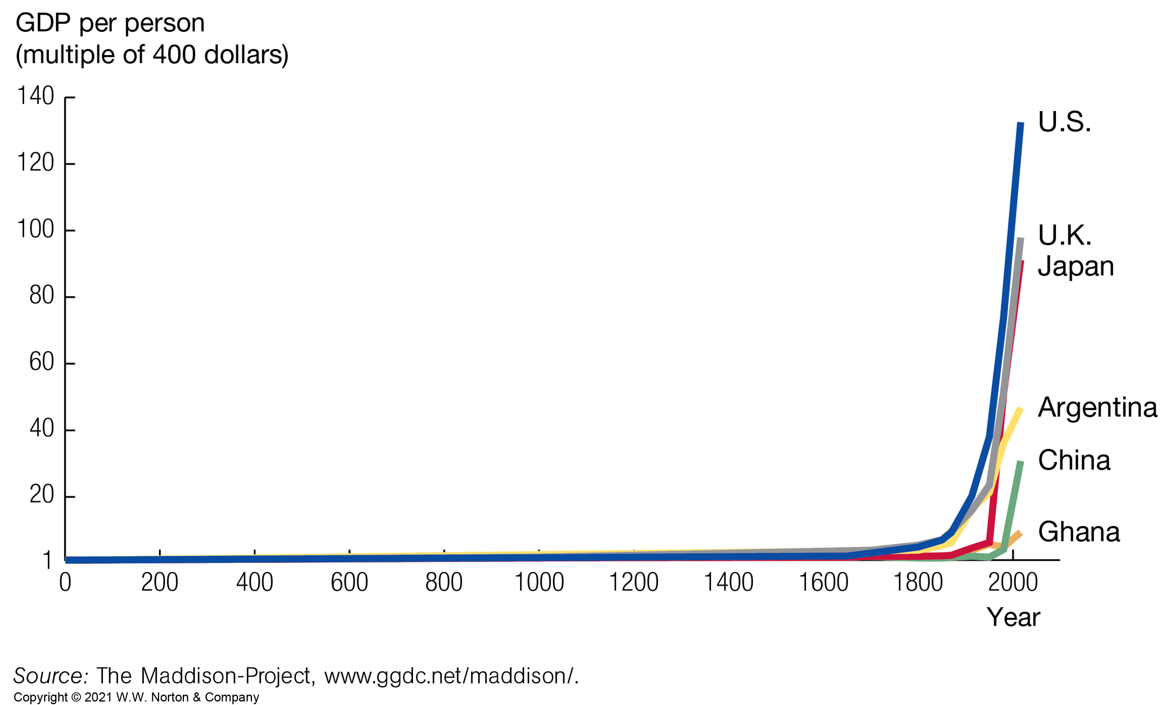
\includegraphics[width=0.6\linewidth]{Figures/long_run_growth}
%	\end{figure}
%	
%\end{frame}

\begin{frame}[wide]{Modern Economic Growth}
	\begin{itemize}
		\item Looking over the past 150 years: from 1870 to 2018, United States \textit{real} per capita GDP rose by more than 15-fold
		\begin{itemize}
			\item On average, around 1870, income per person was around \$3,600 per person (in 2017 dollars)
			\item In 2018, per capita income was about \$61,000.
		\end{itemize}
		\item Assuming this rate of growth continues, a typical college student today will earn a lifetime income about twice that of his or her parents
	\end{itemize}
\end{frame}

\begin{frame}[wide]{Per Capita GDP in the United States, 1870-2020}
	\begin{figure}
		\centering
		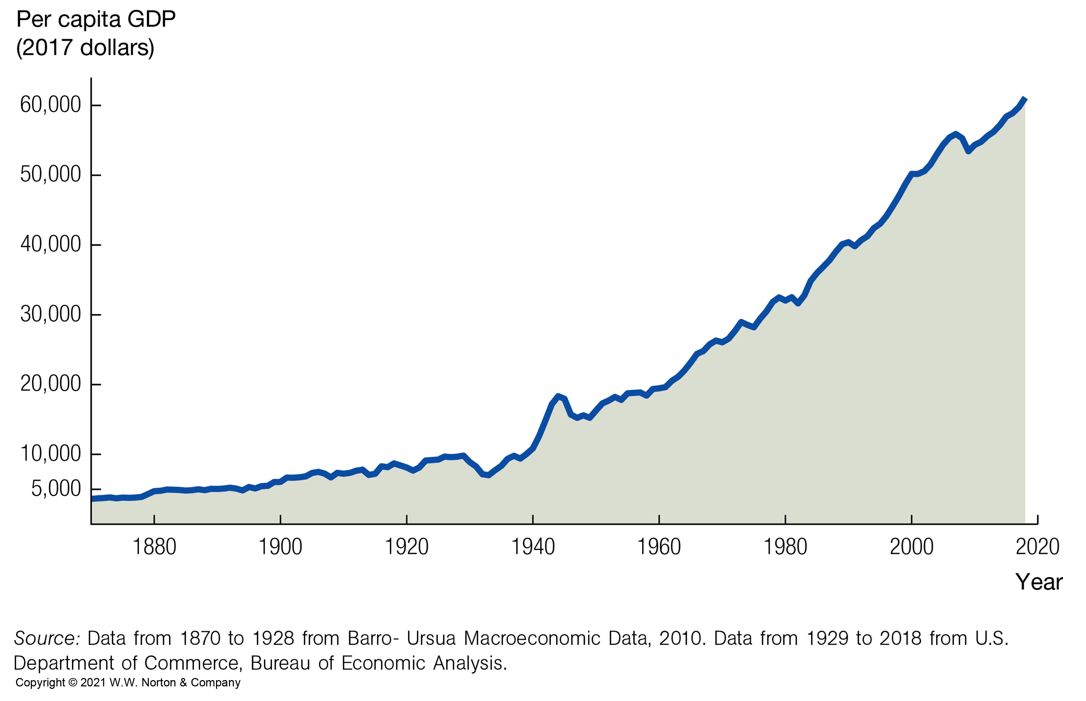
\includegraphics[width=0.6\linewidth]{Figures/US_per_capita_GDP}
	\end{figure}
	
\end{frame}

\begin{frame}[wide]{The Definition of Economic Growth}
	\begin{itemize}
		\item Growth of per capita GDP is the rate of change of per capita GDP
		\begin{itemize}
			\item The goal is to consider how standards of living have changed over time
			\item We could examine the percentage change in the level of GDP, but GDP per capita gives us a better sense of the average person’s income
		\end{itemize}
		\item A percentage change: 
		\[\bar{g} = \frac{y_{t}-y_{t-1}}{y_{t-1}} \text{ so that } y_t = y_{t-1}(1+\bar{g})\]
		where  $\bar{g}$ is the associated constant growth rate (i.e., a parameter)
		
		\item This tells us that the value of GDP per capita today depends on both the value of GDP per capita in the past and the growth rate of GDP per capita
	\end{itemize}
\end{frame}

\begin{frame}[wide]{Example: Population Growth}
	\begin{itemize}
		\item Population growth evolves the same way:
		\[L_{t+1} = L_t (1+\bar{n})\]
		\item Intuitively, tomorrow’s population in time period $t+1$ depends on today's population in period $t$
		\item Then, the period after, we have 
		\[L_{t+2}=L_{t+1}(1+\bar{n})\]
		\item Plug in the first equation into the next one
		\[L_{t+2}=L_t (1+\bar{n})(1+\bar{n}) = L_t (1+\bar{n})^2\]
	\end{itemize}
\end{frame}

\begin{frame}[wide]{Example: Population Growth}
	\begin{itemize}
		\item Continue this process for $t+3$
		\[L_{t+3} = L_{t+2}(1+\bar{n}) =L_{t+1}(1+\bar{n}) (1+\bar{n}) = L_{t}(1+\bar{n}) (1+\bar{n})(1+\bar{n}) \]
		That is, 
		\[L_{t+3} = L_{t}(1+\bar{n})^3 \]
		\item In general, 
		\[L_t = L_0 (1+\bar{n})^t\]
	\end{itemize}
\end{frame}

\begin{frame}[wide]{The Constant Growth Rule}
	\begin{itemize}
		\item The constant growth rule states that
		\[y_t=y_0(1+\bar{g})^t\]
		where 
		\begin{itemize}
			\item $t$ is the time period
			\item $y_t$ is the value of variable $y$ in time $t$
			\item $y_0$ is the initial value of variable $y$ in period 0
			\item $\bar{g}$ is the constant growth rate
		\end{itemize}
	\end{itemize}
\end{frame}

\begin{frame}[wide]{Population over Time}
	\begin{itemize}
		\item Using the formula $L_t=L_0(1+\bar{n})^t$ to compute with $L_0=6$ and $\bar{n}=0.02$ -- roughly the birth rate of the US
		\begin{figure}
			\centering
			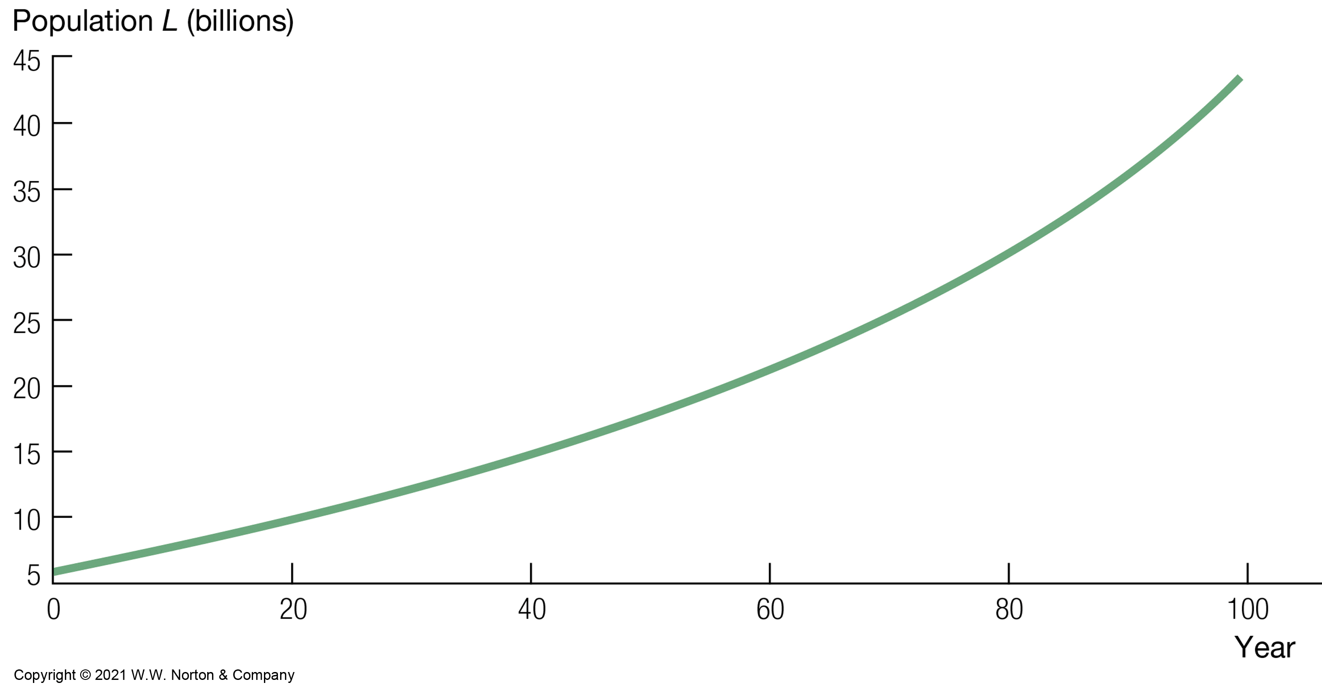
\includegraphics[width=0.7\linewidth]{Figures/pop_over_time_fig_3-3}
		\end{figure}
		
	\end{itemize}
\end{frame}

\begin{frame}[wide]{Compare to the Actual Population in US}
	\begin{itemize}
		\item The shape of the two are similar
		\item But, the calculation we have miss the important event of WWII and population aging
		\begin{figure}
			\centering
			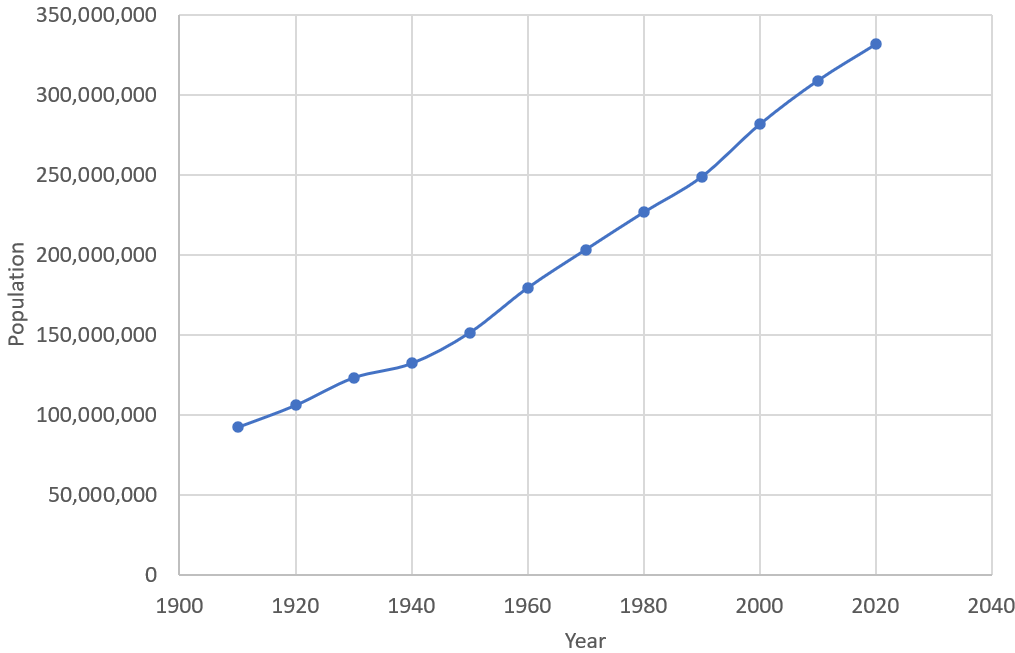
\includegraphics[width=0.7\linewidth]{Figures/us_population_growth}
		\end{figure}
		source: US Census
	\end{itemize}
\end{frame}

%\begin{frame}[wide]{The Rule of 70}
%	\begin{itemize}
%		\item The Rule of 70: If $y$ grows at a rate of $g$ percent per year, then the number of years it takes y to double is approximately equal to $70/g$
%		\item In the other word, it tells us that an economy growing at a constant rate will double every 70/g years
%		\begin{itemize}
%			\item If a country’s income grows at 1 percent per year, it will take about 70 years for income to double
%			\item If growth is at 2 percent per year,	income doubles every 35 = (70/2) years
%			\item Seemingly small differences in growth rates can lead to vastly different outcomes when compounded over time
%		\end{itemize}
%		\item A handy way to calculate when you do not have a calculator, but approximation error
%		\item The time it takes to double only depends on the growth rate and not on the initial value
%		\item The time it takes for income to double depends only on the growth rate, if it is constant, not on the current level of income
%		
%	\end{itemize}
%\end{frame}
%
%\begin{frame}[wide]{The Rule of 70: Derivation}
%	\begin{itemize}
%		\item If income begins at level $y_0$, then we want to know how many years until
%		\[y_t=2\times y_0\]
%		\item Using the constant growth rule
%		\[y_0(1+\bar{g})^t =2\times y_0 \implies (1+\bar{g})^t =2  \]
%		\item Take $\ln$ on both side
%		\[ \ln\left((1+\bar{g})^t\right) =\ln2 \implies t\ln\left(1+\bar{g}\right) =\ln2\]
%		\item Take the approximation that $\ln\left(1+\bar{g}\right) \approx \bar{g}$ and $\ln2 \approx 0.7$, we have
%		\[t\bar{g} = 0.7 \implies t = \frac{0.7}{\bar{g}}\]
%		or, in percentage form,
%		$t = \frac{70}{\bar{g}}$
%	\end{itemize}
%\end{frame}

\begin{frame}[wide]{How to Calculate Constant Growth Rate when it Varies}
	\begin{itemize}
		\item For most of the variables, the growth rate varies over time (e.g., growth in GDP)
		\item Let $g_1=5\%$ and $g_2=2\%$, to calculate the constant growth rate, we want to find
		\[y_0 (1+\bar{g}) (1+\bar{g}) = y_0 (1+0.05)(1+0.02)\]
		\[(1+\bar{g})^2 = (1+0.05)(1+0.02) \implies \bar{g} = \left((1+0.05)(1+0.02)\right)^{1/2} -1 = 0.03489\]
		It is the geometric average of the growth rate across the two year and is consistent with the way of calculating growth rate
	\end{itemize}
\end{frame}

\begin{frame}[wide]{How to Calculate Constant Growth Rate when it Varies}
	\begin{itemize}
		\item How's about taking average of the two growth rate using the "usual" method?
		\[\bar{g} = \frac{g_1+g_2}{2} = \frac{0.05+0.02}{2} = 0.035\]
		The two numbers are close. This is the arithmetic mean.
		\item The two should be close when the growth rate does not varies too much
	\end{itemize}
\end{frame}

\begin{frame}[wide]{Calculating Growth Rates Given Only Two Years of GDP}
	\begin{itemize}
		\item What if we are given data only for the start and end of this series?
		\begin{itemize}
			\item e.g., United States per capita GDP 1870: \$3,600 amd 2018: \$61,000
			
		\end{itemize}
		\item Use the constant growth rule: $y_t=y_0 (1+\bar{g})^t$
			\[\frac{y_t}{y_0} = (1+\bar{g})^t \implies \bar{g} = \left(\frac{y_t}{y_0}\right)^{\frac{1}{t}}-1\]
		\item For example, $\bar{g} = \frac{61000}{3600}^{1/148} - 1 = 0.02$
		\item For $t=1$, 
		\[\bar{g} = \frac{y_1}{y_0}- 1 = \frac{y_1-y_0}{y_0}\]
		The usual percentage change formula
	\end{itemize}
\end{frame}

\begin{frame}[wide]{The Ratio (Logarithmic) Scale}
	\begin{itemize}
		\item From time to time, you may see a plot where the tick marks are not of equal size
		\begin{figure}
			\centering
			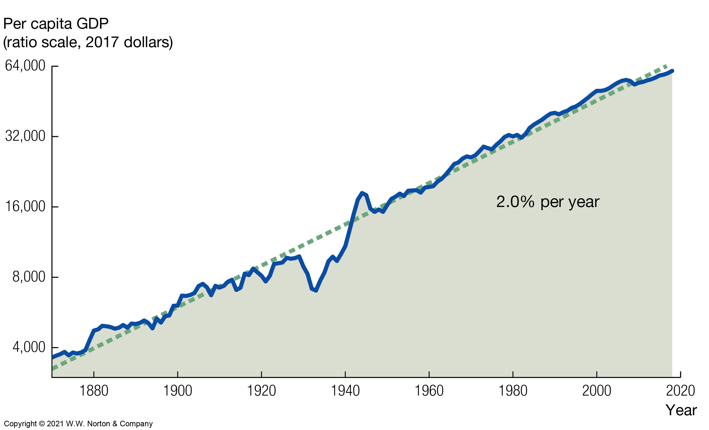
\includegraphics[width=0.7\linewidth]{Figures/ratio_scale}
		\end{figure}
		
	\end{itemize}
\end{frame}

\begin{frame}[wide]{The Ratio (Logarithmic) Scale}
	\begin{itemize}
		\item A plot intervals between tick marks are proportional in terms of ratios rather than absolute differences
		\begin{itemize}
			\item When doubling, we want this constant ratio to be "2." 
			\item e.g., on the y-axis, instead of ``1, 2, 3, 4" we have ''1, 2, 4, 8"
		\end{itemize}
		\item When plotted on a ratio scale, a variable that grows at a constant rate will be a straight line
		\item It is commonly used to represent data where exponential growth or significant variations need to be visually compressed
		\vspace{1mm}
		\begin{itemize}
			\item Using the population growth figure earlier, we cannot tell right away that the growth rate is constant, increasing, or decreasing
		\end{itemize}
	\end{itemize}
\end{frame}

\begin{frame}[wide]{Population over Time, Revisited}
	\begin{itemize}
		\item Absolute population numbers are increasing faster (left), but the rate of growth is staying the same in the right graph because of the linear relationship (right)
	\end{itemize}
	\begin{figure}
		\centering
		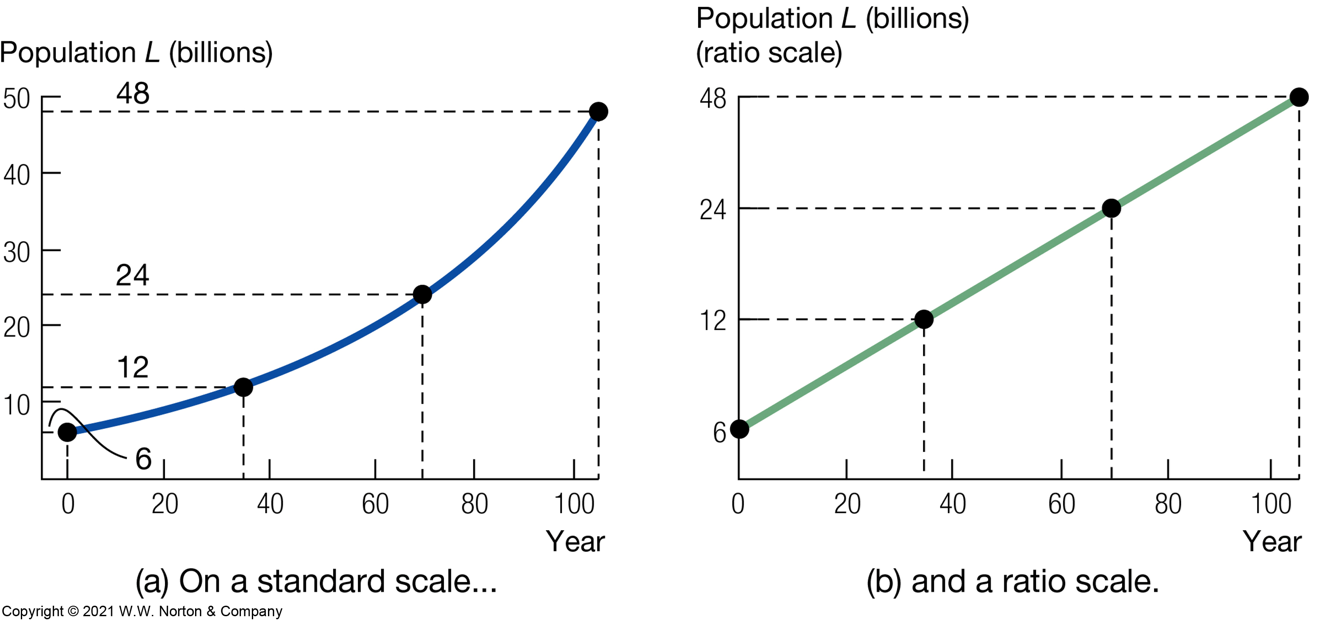
\includegraphics[width=0.7\linewidth]{Figures/ratio_scale1}
	\end{figure}
	
\end{frame}

\begin{frame}[wide]{U.S. GDP on a Ratio Scale}
	\begin{itemize}
		\item On a ratio scale:
		\begin{itemize}
			\item if growth rates are rising, the slope will be increasing
			\item if the growth rate is constant, it will be a straight line
			\item if the growth rate is falling, the slope will be decreasing
		\end{itemize}
		\item Per capita GDP in the United States has grown at approximately 2 percent per year over the past 150 years.
		\begin{itemize}
			\item This outcome is easy to see using a ratio scale
			\item Approximately linear
		\end{itemize}
		
	\end{itemize}
\end{frame}

\begin{frame}[wide]{Per Capita GDP in the United States, Standard vs. Ratio Scale}
	\begin{itemize}
		\item The graph on the left is a standard scale and the one on the right is a ratio scale
		\item Data series lies close to a line that exhibits a constant slope of 2.0 percent per year
		\item To a first approximation, per capita GDP in the United States has been growing at a relatively constant annual rate of 2 percent over the past 150 years
	\end{itemize}
	\begin{figure}
		\centering
		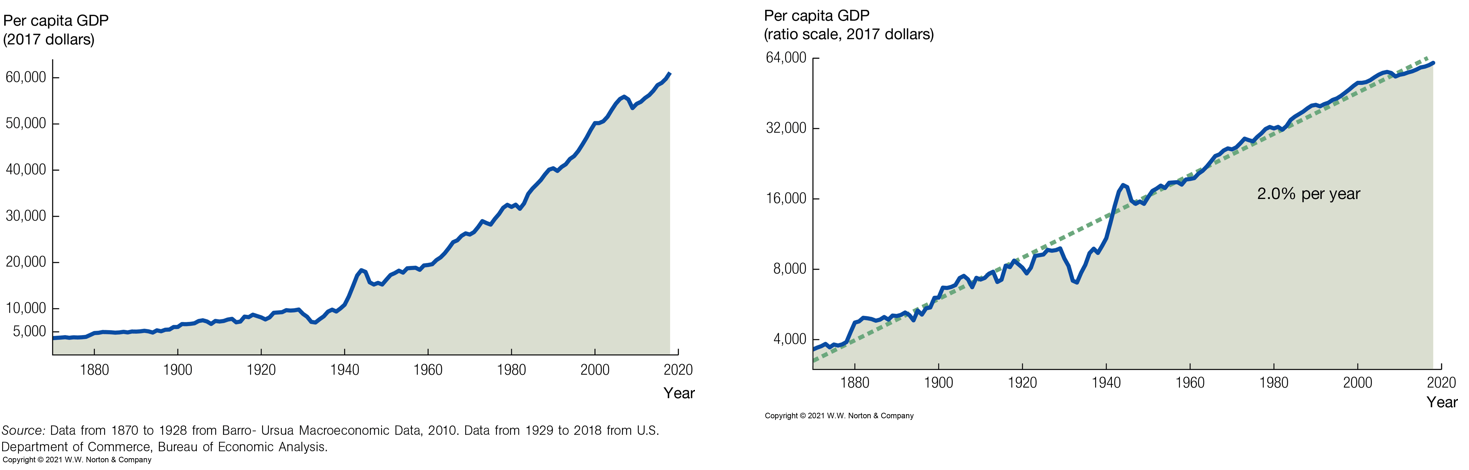
\includegraphics[width=0.8\linewidth]{Figures/US_GDP_ratio_scale}
	\end{figure}
	
\end{frame}

\begin{frame}[wide]{The Ratio Scale in Action: Per Capita GDP since 1870}
	\begin{itemize}
		\item The picture contains more information, but we have to read it carefully
		\item The per capita income line is flag for the UK relative to the US until the 50s
		\item From 1880 to 1920, Argentina grew rapidly; Since 1980, growth has slowed considerably
		\begin{figure}
			\centering
			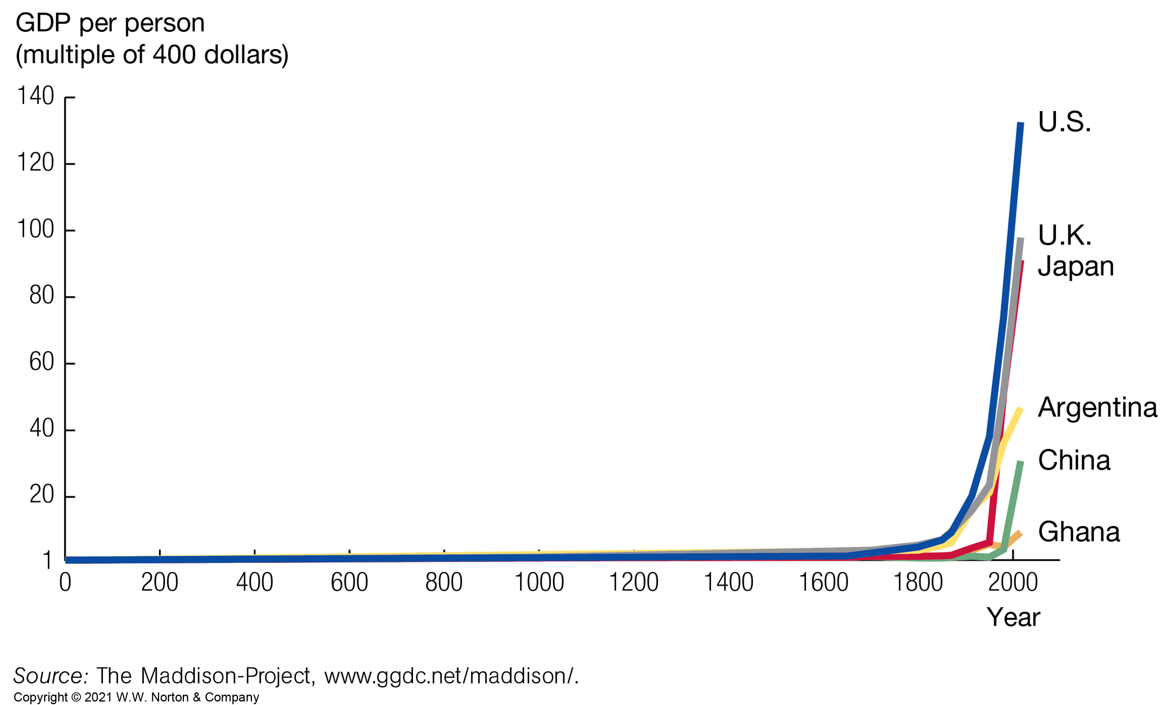
\includegraphics[width=0.45\linewidth]{Figures/long_run_growth}
			\includegraphics[width=0.45\linewidth]{"Figures/The Ratio Scale in Action"}
		\end{figure}
	\end{itemize}
\end{frame}

%\begin{frame}[wide]{Modern Growth around the World}
%	\begin{itemize}
%		\item In the late nineteenth century, the United Kingdom was the richest country in the world, but it start grew substantially more slowly than the United States in the 20th century
%		\item After World War II, growth in Germany and Japan were similar, in that they both accelerated
%		\item Argentina had accelerated growth until 1980 and then slowed considerably
%		\item China, Vietnam and India have start ``converging'' recently
%		\item Convergence:
%		\begin{itemize}
%			\item Poorer countries will grow faster to “catch up” to the level of income in richer countries
%		\end{itemize}
%	\end{itemize}
%\end{frame}
%
%\begin{frame}[wide]{A Broad Sample of Countries}
%	\begin{itemize}
%		\item Over the period 1960--2017:
%		\begin{itemize}
%			\item Some countries have displayed negative growth rates.
%			\item Other countries have maintained growth rates of nearly 7\%.
%			\item Most countries have maintained approximately 2\% growth rates.
%			\item Small variances in growth rates lead to significant differences in standards of living.
%		\end{itemize}
%	\end{itemize}
%\end{frame}
%
%\begin{frame}[wide]{Levels and Growth Rates of Per Capita GDP}
%	\begin{itemize}
%		\item From 1960 to 2017, growth rates ranged from -2 percent to +7 percent per year
%		\item South Korea, Egypt, Thailand, Botswana, and Japan grew the fastest over this period
%		\item Central African Republic, the Democratic Republic of the Congo, Niger, and Guinea all had negative average growth
%		\begin{figure}
%			\centering
%			\includegraphics[width=0.6\linewidth]{"../Week 4/Figures/Levels and Growth Rates of Per Capita GDP"}
%		\end{figure}
%		
%	\end{itemize}
%\end{frame}
%
%\begin{frame}[wide]{Case Study: People versus Countries}
%	\begin{itemize}
%		\item Compare 2017 to 1960, the bulk of the world’s population is substantially richer and  the fraction of people living in poverty has fallen
%		\item A major reason for changes:
%		\begin{itemize}
%			\item Economic growth in China and India
%			\item These two countries account for 40 percent of the world population
%		\end{itemize}
%	\end{itemize}
%	\begin{figure}
%		\centering
%		\includegraphics[width=0.5\linewidth]{"../Week 4/Figures/People versus Countries"}
%	\end{figure}
%	
%\end{frame}
%
%\begin{frame}[wide]{Some Useful Properties of Growth Rates}
%	\begin{itemize}
%		\item A lot of time we have economic variables express in term of some mathematical combination of other variables (e.g., GDP per Capita)
%		\item Growth rates of ratios, products, and powers follow several (approx.) simple rules
%		\item Suppose two variables $x$, $y$ and $z$ have average annual growth rates of $g_x$, $g_y$ and $z$, respectively. Then
%		\vspace{1mm}
%		\[\text{If } z=x/y \text{, then  } g_z=g_x-g_y\]
%		\vspace{1mm}
%		\[\text{If } z=x\times y \text{, then  } g_z=g_x+g_y\]
%		\vspace{1mm}
%		\[\text{If } z=x^a \text{, then  } g_z=a \times g_x\]
%		\item We can combine these rules 
%	\end{itemize}
%\end{frame}
%
%\begin{frame}[wide]{Examples of Growth Rate Calculations}
%	\begin{figure}
%		\centering
%		\includegraphics[width=0.7\linewidth]{"../Week 4/Figures/Examples of Growth Rate"}
%	\end{figure}
%	
%\end{frame}
%
%\begin{frame}[wide]{U.S. Population, GDP, and Per Capita GDP}
%	\begin{itemize}
%		\item Total GDP = GDP per capita $\times$ number of workers,
%		\item Growth rate of total GDP = growth rate of per capita GDP + the growth rate of the population
%		\begin{figure}
%			\centering
%			\includegraphics[width=0.5\linewidth]{"../Week 4/Figures/U.S. Population, GDP, and Per Capita GDP"}
%		\end{figure}
%		
%	\end{itemize}
%\end{frame}
%
%\begin{frame}[wide]{Example: Growth Rules with Cobb Douglas Production Function}
%	\begin{itemize}
%		\item Applying rules of growth rates to a Cobb Douglas production function (see Ch.4):
%		\[Y_t = A_t K_t^{1/3} L_t^{2/3}\]
%		\item It says the output depends on the levels of technology, capital, and labor. Its growth rate of output can be decomposed into growth rate of a productivity term A,	contributions to growth from capital K, and labor L
%		\item Using $\text{If } z=x\times y \text{, then  } g_z=g_x+g_y$,
%		\[g(y) = g(A) + g(K^{1/3}) + g(L^{2/3})\]
%		\item Then, use $\text{If } z=x^a \text{, then  } g_z=a \times g_x$, 
%		\[g(y) = g(A) + \frac{1}{3}g(K) + \frac{2}{3} g(L)\]
%	\end{itemize}
%\end{frame}
%
%\begin{frame}[wide]{The Benefits and Costs of Economic Growth}
%	\begin{itemize}
%		\item The benefits of economic growth:
%		\begin{itemize}
%			\item Improvements in health
%			\item Higher incomes
%			\item Increase in the variety of goods and services
%		\end{itemize}
%		\item Costs of economic growth include:
%		\begin{itemize}
%			\item Environmental problems
%			\item Income inequality across and within countries
%			\item Loss of certain types of jobs
%		\end{itemize}
%		\item	Economists generally have a consensus that the benefits of economic growth outweigh the costs.
%	\end{itemize}
%\end{frame}

\begin{frame}[wide]{Next Lecture}
	\begin{itemize}
		\item Next lecture will finish Ch.3 and start covering Ch.4
	\end{itemize}
\end{frame}

\end{document}